%----------------------------------------------------------------------------------------
%	PACKAGES AND THEMES
%----------------------------------------------------------------------------------------
\documentclass[aspectratio=169,xcolor=dvipsnames, t]{beamer}
\usepackage{fontspec} % Allows using custom font. MUST be before loading the theme!
\usetheme{SimplePlus}
\usepackage[spanish,es-tabla]{babel}
\selectlanguage{spanish}
\usepackage{hyperref}
\usepackage{graphicx} % Allows including images
\usepackage{booktabs} % Allows the use of \toprule, \midrule and  \bottomrule in tables
\usepackage{svg} %allows using svg figures
\usepackage{tikz}
\usepackage{makecell}
\usepackage{wrapfig}
% ADD YOUR PACKAGES BELOW

%----------------------------------------------------------------------------------------
%	TITLE PAGE CONFIGURATION
%----------------------------------------------------------------------------------------

\title[Prompt sentiment]{GII\_O\_MA\_23.23. Aplicación de análisis de reseñas basado en modelos de lenguaje grandes mediante prompt engineering.} % The short title appears at the bottom of every slide, the full title is only on the title page
\subtitle{Trabajo de fin de grado del Grado Ingeniería Informática (Online) en la Universidad de Burgos}

\author[García Sánchez]{Teodoro Ricardo García Sánchez}
\institute[Grado de Ingeniería Informática (Online)]{Dra. Virginia Ahedo García\\Dr. José Ignacio Santos Martín}


\date{14 de Febrero de 2024} % Date, can be changed to a custom date
%----------------------------------------------------------------------------------------
%	PRESENTATION SLIDES
%----------------------------------------------------------------------------------------

\begin{document}

\maketitlepage

\begin{frame}[t]{Contenido}
    \tableofcontents
\end{frame}

%------------------------------------------------
% Section divider frame
\makesection{Introducción}

%------------------------------------------------
% Bullets
\begin{frame}{El análisis de sentimientos}
    \begin{itemize}
        \item Intenta descubrir la actitud de un usuario con respecto a algún tema
        \item Esta puede ser una reseña, un estado afectivo o emocional
        \item También se denomina minería de opinión
        \item Clasifica la polaridad de un texto
        \item Vamos a utilizar ``Prompt engineering'' en este trabajo (LLM)
        \item Evaluaremos su precisión
    \end{itemize}
\end{frame}

%------------------------------------------------
% Section divider frame
\makesection{Objetivos del proyecto}

%------------------------------------------------
% Bullets
\begin{frame}{Prompt engineering y análisis de sentimiento}
    \begin{itemize}
        \item Crear una aplicación que utilice modelos de lenguaje grandes (como ChatGPT, Bard o Llama) de manera efectiva para analizar y comprender las reseñas de usuarios.
        \item Diseñar un sistema basado en ``\emph{prompts}'', definiendo las tareas, entradas y salidas de la respuesta a una instrucción, para lograr una solución ágil sin necesidad de nuevos entrenamientos.
        \item Relacionar opiniones y emociones con calificaciones
        \item Implementar técnicas de ``\emph{prompt engineering}''
    \end{itemize}
\end{frame}

%------------------------------------------------
% Section divider frame
\makesection{Conceptos teóricos}

%------------------------------------------------
% Bullets
\begin{frame}{Análisis sentimiento, PLN y Patrones}
    \begin{itemize}
        \item Análisis de sentimiento
        \item Procesamiento de lenguaje natural
        \item Prompt Engineering
        \item Patrones de diseño
    \end{itemize}
\end{frame}

%------------------------------------------------
% Section divider frame
\makesection{Técnicas y herramientas}

%------------------------------------------------
% Técnicas
\begin{frame}{Técnicas}
    \begin{itemize}
        \item ORM
        \item MVC
        \item LLM
    \end{itemize}
\end{frame}

%------------------------------------------------
% ORM

\begin{frame}{ORM}
\begin{figure}
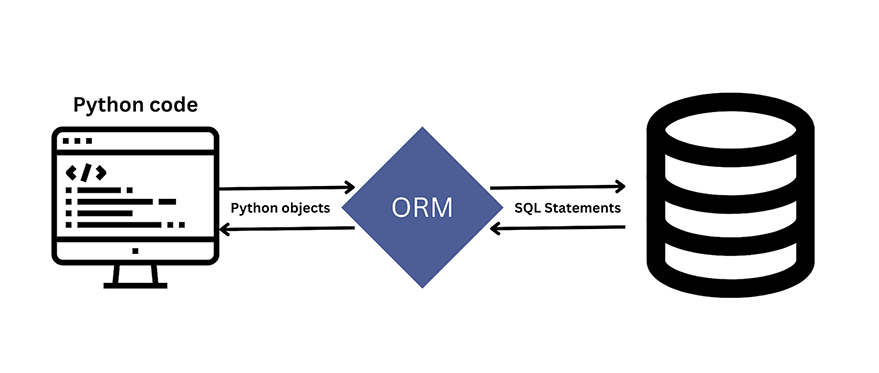
\includegraphics[width=8cm]{style_data/img/orm.png}
\centering
\end{figure}
\end{frame}


%------------------------------------------------
% MVC
\begin{frame}{MVC}
\begin{figure}[t]
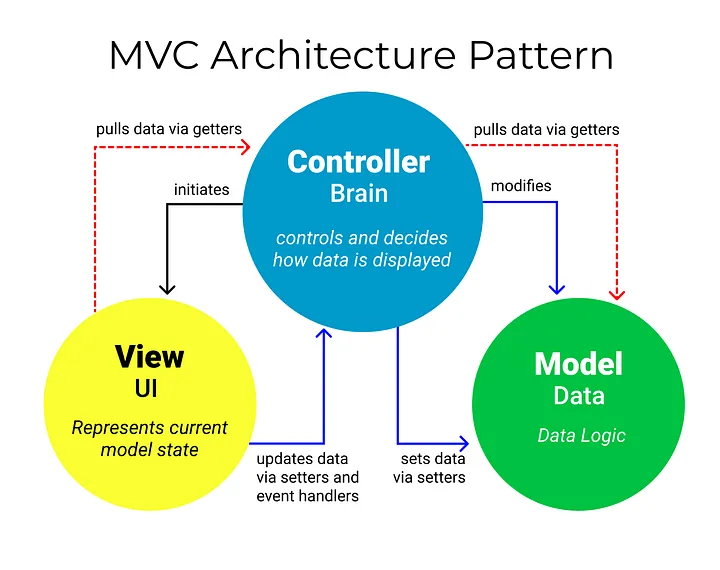
\includegraphics[width=7cm]{style_data/img/mvc_pattern.png}
\centering
\end{figure}
\end{frame}

%------------------------------------------------
% LLM
\begin{frame}{LLM}
\begin{figure}

\includegraphics[width=8cm]{style_data/img/llm.jpg}
\centering
\end{figure}
\end{frame}

%------------------------------------------------
% Herramientas
\begin{frame}{Herramientas}
    \begin{itemize}
        \item Python
        \item Flask
        \item SQLAlchemy
        \item Docker
        \item PostgreSQL
        \item ChatGPT/OpenAI
        \item LlamaCpp
    \end{itemize}
\end{frame}

%------------------------------------------------
% Python, Flask, SQLAlchemy, PostgreSQL
\begin{frame}{Python, Flask, SQLAlchemy, PostgreSQL}
\begin{figure}
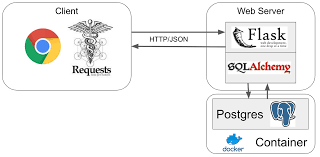
\includegraphics[width=8cm]{style_data/img/python_flask.png}
\centering
\end{figure}
\end{frame}

%------------------------------------------------
% Docker
\begin{frame}{Docker}
\begin{figure}
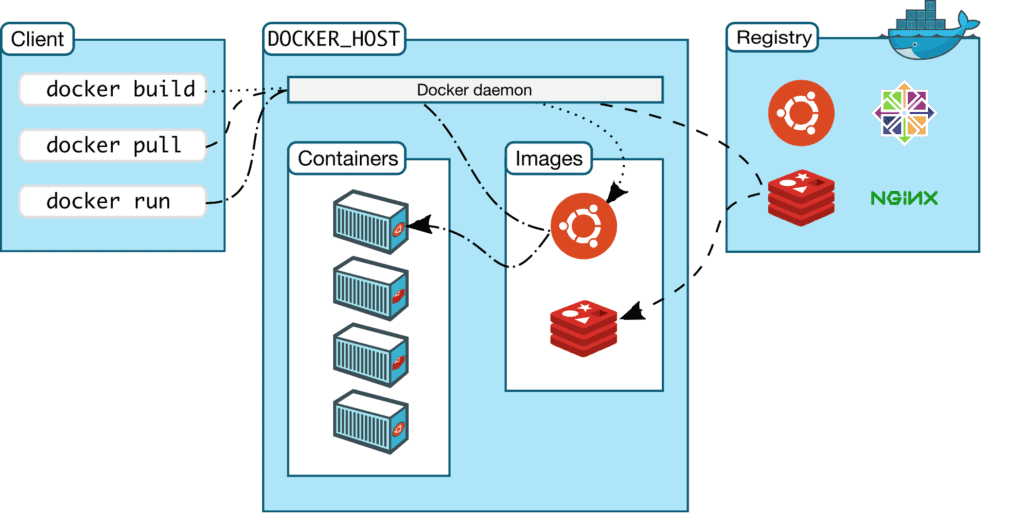
\includegraphics[width=8cm]{style_data/img/ArquiteturaDocker.png}
\centering
\end{figure}
\end{frame}

%------------------------------------------------
% Aspectos generales
\makesection{Aspectos relevantes del desarrollo del proyecto}

%------------------------------------------------
% Metodologías
\begin{frame}{Metodologías I}
        \begin{figure}
            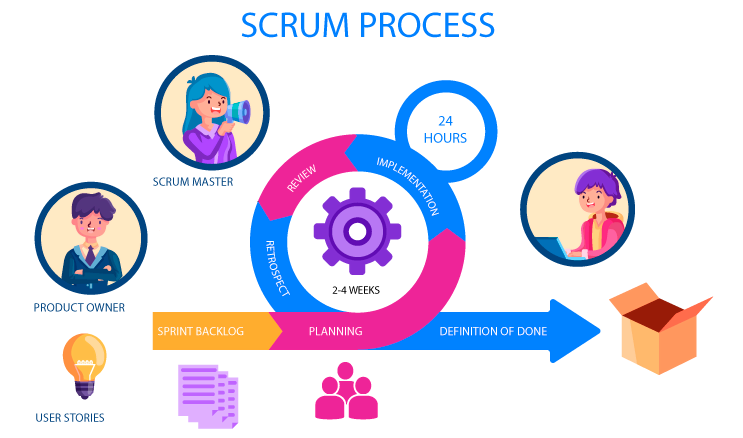
\includegraphics[width=8cm]{style_data/img/scrum-methodology.png}        
            \caption{Scrum}
            \label{fig:subim1}
        \end{figure}
\end{frame}

\begin{frame}{Metodologías II}
    
    \begin{figure}
        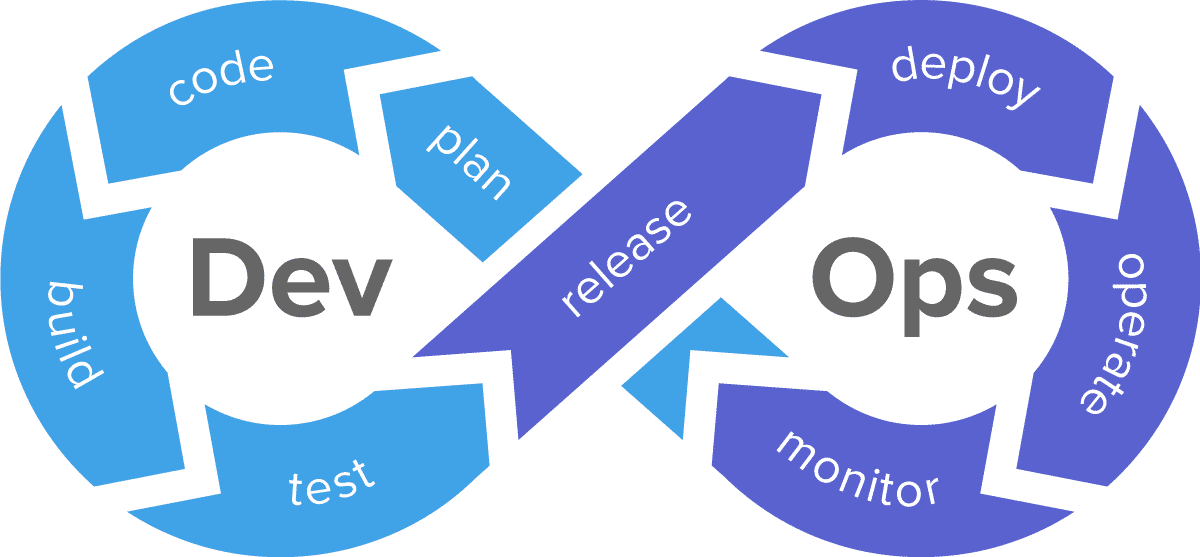
\includegraphics[width=8cm]{style_data/img/dev-ops.png}        
        \caption{DevOps}
        \label{fig:subim2}
    \end{figure}
    
\end{frame}

%------------------------------------------------
% Bullets
\begin{frame}{Desarrollo del proyecto}
    \begin{itemize}
        \item Elección del modelo
        \item Elección del conjunto de datos
        \item Diseño del prompt
        \item Validación del sistema
    \end{itemize}
\end{frame}

%------------------------------------------------
% Section divider frame
\makesection{Trabajos relacionados}

%------------------------------------------------
% Bullets
\begin{frame}{Trabajos relacionados}
    \begin{itemize}
        \item Lingmotif
        \item Lexalytics
        \item IBM Watson Studio
        \item Sentinel
        \item Free Sentiment Analysis   
    \end{itemize}
\end{frame}

%------------------------------------------------
% Section divider frame
\makesection{Conclusiones y Líneas de trabajo futuras}

%------------------------------------------------
% Bullets
\begin{frame}{Conclusiones}
    El uso de modelos grandes de lenguaje está cada vez más extendido en muchos sectores tecnológicos.
En estos momentos hay una explosión de proyectos y usos que no eramos capaces de imaginarnos hace un años.
En este trabajo se han combinado estas técnicas con otras más tradicionales para conseguir una aplicación 
útil con muchas oportunidades de mejora y ampliación.
Lo que he intentado es establecer una plataforma que sea flexible para poderla ampliar y escalar tanto como se necesite.
En el camino he aprendido desde el uso de LLMs, Python, servicios web, seguridad (mediante tokens), 
despliegue continuo con docker, etc. El resultado creo que es una aplicación sencilla pero 
con mucho potencial y suficientemente flexible como para servir de base de otros desarrollos más complejos.
\end{frame}

%------------------------------------------------
% Bullets
\begin{frame}{Líneas de trabajo futuras}
    \begin{itemize}
        \item Nuevos modelos
        \item Más opciones para importar conjunto de datos
        \item Permitir al usuario modificar el ``{prompt}'' para incluir más funcionalidades
        \item Gestión de ficheros
    \end{itemize}
\end{frame}

%------------------------------------------------
% Section divider frame
\makesection{Bibliografía}
%------------------------------------------------
% Refenrenced
\begin{frame}{}
    % Beamer does not support BibTeX so references must be inserted manually as below
    \footnotesize{
        \begin{thebibliography}{99}
            \bibitem[Smith, 2012]{p1} John Smith (2012)
            \newblock Title of the publication
            \newblock \emph{Journal Name} 12(3), 45 -- 678.

            \bibitem[Doe, 2012]{p1} Joe Doe (2012)
            \newblock Title of the publication
            \newblock \emph{Journal Name} 12(3), 45 -- 678.
            \bibitem[Doe, 2013]{p} Jane Doe (2012)
            \newblock Title of the publication
            \newblock \emph{Journal Name} 12(3), 45 -- 678.
        \end{thebibliography}
    }
\end{frame}

%----------------------------------------------------------------------------------------
% Final PAGE
% Set the text that is showed on the final slide
\finalpagetext{Demostración}
%----------------------------------------------------------------------------------------
\makefinalpage
%----------------------------------------------------------------------------------------
\end{document}